\documentclass[11pt,letterpaper]{article}
\usepackage[margin=0.76in]{geometry}
\usepackage{mathptmx}
\usepackage[T1]{fontenc}
\usepackage[utf8]{inputenc}
\usepackage{amsmath,amssymb}
\usepackage{graphicx}
\usepackage{booktabs}
\usepackage{tabularx}
\usepackage{array}
\usepackage{xcolor}
\usepackage{xurl}
\usepackage{hyperref}
\usepackage{caption}
\usepackage[numbers,sort&compress]{natbib}
\usepackage{microtype}
\usepackage{ragged2e}

\hypersetup{
  colorlinks=true,
  linkcolor=blue!60!black,
  citecolor=blue!60!black,
  urlcolor=blue!60!black
}

\captionsetup{font=small,labelfont=bf}
\newcolumntype{L}[1]{>{\RaggedRight\arraybackslash}p{#1}}
\newcolumntype{C}[1]{>{\Centering\arraybackslash}p{#1}}
\newcolumntype{Y}{>{\RaggedRight\arraybackslash}X}
\setlength{\parskip}{0.36em}
\setlength{\parindent}{0pt}
\renewcommand{\topfraction}{0.88}
\renewcommand{\bottomfraction}{0.85}
\renewcommand{\textfraction}{0.08}
\renewcommand{\floatpagefraction}{0.75}
\sloppy

\title{\textbf{Systematic False-Positive Secondary Findings from ClinVar VCF Inheritance Stripping and Condition Pollution Across Six Open-Source ACMG SF Pipelines}}

\author{
  Computational Clinical Genomics Audit Working Group\\
  \small\textit{Brief Communication / Technical Analysis --- Fully Reproducible Benchmark \& Execution Package}
}
\date{November 25, 2026}

\begin{document}
\maketitle

\begin{abstract}
\noindent
Clinical exome and genome sequencing programs routinely screen patient VCFs for medically actionable autosomal-dominant (AD) secondary findings (ACMG SF v3.3; 84 genes, 73 AD) by matching against NCBI ClinVar pathogenic and likely pathogenic (P/LP) annotations. However, official ClinVar VCF files (\texttt{clinvar.vcf.gz}) omit submission-level mode-of-inheritance tags (\texttt{ModeOfInheritance}) and collapse multi-submitter disease names (\texttt{CLNDN}/\texttt{CLNDISDB}) into unstratified unions. Here we execute six independent, publicly released ACMG SF filtering pipelines spanning R, Python, and compiled Rust (\texttt{OwnGenome}, \texttt{CPSR v2.4.0}, \texttt{SFtool}, SickKids \texttt{CPHI-DRAGEN-anno}, \texttt{viking-genes}, and \texttt{DNA}) plus a seventh clinical MOI validator (\texttt{Talos v12.3.1}) on a live-SCV-verified 24-variant GRCh38 heterozygous (\texttt{0/1}) benchmark panel. All 6/6 executed pipelines emit false-positive AD secondary findings on dual-mode and opposite-mechanism alleles. Even the three engineered pipelines achieving 4/4 (100\%) specificity on pure-recessive heterozygous negative controls (\texttt{MUTYH}, \texttt{ATP7B}, \texttt{HFE}, \texttt{GAA}) and 4/4 sensitivity on AD controls emitted 13/15 to 14/15 (86.7--93.3\%) false positives, including 3/3 locked recessive \textit{RYR1} congenital myopathy alleles. Notably, compiled Rust \texttt{OwnGenome} rejected 7 \textit{RYR1}/\textit{APOB}/\textit{RET}/\textit{DES} truncating alleles as non-qualifying \texttt{HIGH}-impact loss-of-function variants while simultaneously returning all 7 exact alleles as active \texttt{clinvar\_hits}---6 silently (\texttt{condition\_not\_acmg=false}) because aggregate \texttt{CLNDN} pollution defeated its own phenotype-warning logic. Across gnomAD v4.1 joint summary frequencies (807,162 individuals: 730,947 exomes, 76,215 genomes; evaluated as cumulative variant-level carrier-instance rates [Boole upper bound], independence-model prevalence estimates, and model-free single-variant lower bounds rather than exact deduplicated individual counts), these pipeline architectures yield 1.72--2.17 high-callability ($\ge 80\%$ AN) 2--4$\star$ false-positive AD variant-return instances per 1,000 diploid sample-equivalents (5.30--6.59\% of emitted calls; independence-model estimate 1.72--2.17/1,000; 1.23--1.48/1,000 at $\ge 95\%$ AN). An exhaustive live ClinVar XML audit of all 69 3$\star$ Expert-Panel \textit{RYR1} alleles in gnomAD v4.1 shows that 10/69 (14.5\%) are strictly autosomal-recessive Congenital Myopathies VCEP curations comprising 30.8\% (424/1,377) of 3$\star$ \textit{RYR1} heterozygous instances---83.2\% (153/184) in South Asians and 57.4\% (39/68) in Africans, with 98.6\% (418/424) polluted by \texttt{OMIM:145600} (malignant hyperthermia). In \textit{APOB}, 35.4\% of raw 2--4$\star$ P/LP instances (429/1,213; 37.5\% AN-normalized rate share) are cardioprotective low-LDL hypobetalipoproteinemia pLoFs misreturned as high-LDL familial hypercholesterolemia. Even after \textit{TTN} high-PSI ($>90\%$) filtering, \texttt{OwnGenome} exhibits a 2.51-fold South Asian-to-European false-positive disparity at $\ge 80\%$ AN (4.10 vs.\ 1.63/1,000; model-free SAS lower bound 3.34/1,000 from \textit{RYR1} p.Arg3550Trp alone; 3.46-fold at $\ge 95\%$ AN). A validated four-layer downstream patch incorporating ClinGen \texttt{lof=no} ClinVar gating with AD Expert-Panel override (preserving NMD-escaping \textit{TNNT2} p.Trp297Ter) and SCV-level MOI filtering cuts benchmark false positives from 13--15/15 to 1/15 while retaining 100.0\% (1,533/1,533) of genuine 3$\star$ AD Expert-Panel alleles, motivating upstream ClinVar VCF \texttt{CLNMOI} emission.
\end{abstract}

\section{Introduction}
Opportunistic return of secondary findings under the ACMG SF v3.3 policy (84 genes; 73 autosomal dominant [AD], 8 autosomal recessive [AR], 3 X-linked) is now embedded in clinical exome/genome pipelines and national biobanks worldwide~\citep{lee2025acmgsf33,kerr2025viking}. Recent large-scale audits have evaluated allele-frequency cutoffs for ACMG SF genes~\citep{johnston2026daft} and penetrance of predicted loss-of-function (pLoF) variants in gnomAD v4~\citep{gudmundsson2025gnomad}, confirming that 2--4$\star$ ClinVar P/LP alleles rarely violate BA1 frequency ceilings. Yet as of our logged prior-art search on November 25, 2026 (PubMed, Europe PMC, and OpenAlex; search log archived in \texttt{literature\_search\_log\_phase2.json}), no published study was retrieved that empirically executed open-source ACMG SF software pipelines to benchmark \textit{allelic pleiotropy, dual mode of inheritance (MOI), and directional mechanism inversion inside AD-listed ACMG SF genes} (bounded by database indexing and query scope; absence of retrieval does not establish absolute priority).

Multiple AD-listed ACMG SF v3.3 genes harbor ClinVar P/LP alleles that do not cause the ACMG-targeted AD phenotype in heterozygotes: (i) \textit{RYR1}, listed exclusively for AD gain-of-function (GoF) malignant hyperthermia susceptibility (MHS, \texttt{OMIM:145600})~\citep{johnston2021ryr1vcep}, also harbors hundreds of AR congenital myopathy missense and pLoF alleles curated by the ClinGen Congenital Myopathies Variant Curation Expert Panel (VCEP); (ii) \textit{TTN}, restricted by ACMG SF footnote~f to truncating variants in constitutively expressed cardiac exons (PSI~$>90\%$)~\citep{roberts2015ttn,lee2025acmgsf33}, contains non-truncating and low-PSI skeletal-myopathy alleles; (iii) \textit{APOB}, listed for AD familial hypercholesterolemia (FH, elevated LDL-C via receptor-binding missense alleles), contains pLoF alleles causing familial hypobetalipoproteinemia (FHBL, \texttt{OMIM:615558})---which \emph{lowers} LDL-C and is cardioprotective; and (iv) \textit{RET} (GoF MEN2 thyroid cancer vs.\ LoF Hirschsprung disease), \textit{DES}/\textit{CACNA1S} (dominant-negative/GoF AD vs.\ AR null alleles), \textit{LMNA} (cardiac DCM vs.\ AR neuropathy), and \textit{VHL} (AD cancer vs.\ AR Chuvash erythrocytosis).

Crucially, inspecting raw NCBI ClinVar GRCh38 VCF headers (\texttt{clinvar.vcf.gz}, \texttt{\#\#fileDate=2026-11-22})~\citep{landrum2025clinvar} reveals two upstream schema defects: (1) zero of the 31 \texttt{\#\#INFO} tags encode \texttt{ModeOfInheritance}, stripping SCV-level XML inheritance assertions entirely; and (2) \texttt{CLNDN} and \texttt{CLNDISDB} aggregate every submitter's disease strings into an unstratified union, allowing a single legacy gene-level submission to pollute an AR-only allele with AD OMIM identifiers. Whether deployed open-source ACMG SF pipelines actually succumb to these defects---or already exclude such alleles via curated lists, mechanism rules, or disease matching---remains an empirical software-execution question.

\section{Methods}
\subsection{Locked 24-Variant GRCh38 Heterozygous Benchmark Panel}
Before inspecting external pipeline code, we locked a falsification protocol requiring execution of real, publicly versioned clinical SF software (no synthetic toy filters). We extracted 24 real GRCh38 ClinVar P/LP alleles directly from \texttt{clinvar.vcf.gz} (\texttt{2026-11-22}), constructed a standardized high-confidence heterozygous (\texttt{0/1}, \texttt{GQ=99}, \texttt{DP=40}, \texttt{AD=20,20}) VEP-CSQ + ClinVar VCF, and verified SCV-level \texttt{ModeOfInheritance} and VCEP identity via live NCBI E-utilities VCV XML queries:
\begin{itemize}\setlength{\itemsep}{1.5pt}
  \item \textbf{Core 3 locked AR-in-AD \textit{RYR1} alleles:} \texttt{19-38527014-C-T} (p.Arg3550Trp, 3$\star$ ClinGen Congenital Myopathies VCEP \texttt{MOI=AR}), \texttt{19-38523211-C-G} (c.10348-6C$>$G, 3$\star$ Congenital Myopathies VCEP \texttt{MOI=AR}), and \texttt{19-38505338-CAT-C} (p.Ile2781fs, 2$\star$ P frameshift pLoF). All three carry polluted \texttt{OMIM:145600} MH tags in \texttt{CLNDN}/\texttt{CLNDISDB}.
  \item \textbf{Honest self-correction control (1 allele):} \texttt{2-178568947-T-A} (\textit{TTN} p.Lys25729Ter, 2$\star$ LP), initially hypothesized as AR-only, was verified against Cardiodb left-ventricular exon PSI intervals to lie inside a constitutive high-PSI ($>90\%$) A-band exon (\texttt{chr2:178525987-178622769}) and honestly reclassified as an ambiguous/AD-eligible \textit{TTN}tv.
  \item \textbf{Expanded 12 verified discordant alleles:} 4 additional AR \textit{RYR1} alleles (including 3 with zero MH tag in \texttt{CLNDN}), 2 \textit{TTN} non-SF alleles (low-PSI $\le 90\%$ nonsense p.Gln12085Ter; AR missense p.Trp34072Arg), 2 opposite-direction \textit{APOB} low-LDL pLoFs (p.Gly3617fs, p.Arg439Ter), 1 opposite-mechanism \textit{RET} Hirschsprung nonsense (p.Glu238Ter), 1 \textit{DES} AR null (p.Thr76fs), 1 \textit{LMNA} CMT2 neuropathy missense (p.Arg48Gly), and 1 \textit{VHL} Chuvash polycythemia allele (p.Arg200Leu).
  \item \textbf{Controls (8 alleles):} 4 verified AD positive controls (3$\star$ MHS VCEP \textit{RYR1} p.Gly2434Arg, high-PSI A-band \textit{TTN} p.Arg20626Ter, 3$\star$ \textit{BRCA1} p.Glu23fs, 3$\star$ \textit{LDLR} p.Cys231Trp) and 4 pure-AR heterozygous negative controls (\textit{MUTYH} p.Gly368Asp, \textit{ATP7B} p.His1069Gln, \textit{HFE} p.Cys282Tyr, \textit{GAA} c.-32-13T$>$G).
\end{itemize}

\subsection{Direct Execution of Six Public ACMG SF Pipelines}
We shallow-cloned pinned releases of six independent public pipelines and executed their unmodified core SF selection code directly on the 24-variant panel: (1) \texttt{GeiserX/OwnGenome} (\texttt{c324b61}, Rust binary compiled via \texttt{cargo build --release --bin og} and executed with \texttt{og summary collect --only b}); (2) \texttt{sigven/cpsr} \texttt{v2.4.0} (\texttt{7f68f9d}, Oslo University Hospital~\citep{nakken2021cpsr}, R \texttt{retrieve\_\allowbreak secondary\_\allowbreak calls()}); (3) \texttt{babelomics/SFtool} (\texttt{0d72249}, Andalusian Health System, Python \texttt{pr\_\allowbreak variant\_\allowbreak selection()}); (4) \texttt{ccmbioinfo/CPHI-DRAGEN-anno} (\texttt{974860d}, SickKids Toronto, Python \texttt{add\_\allowbreak acmg\_\allowbreak sf\_\allowbreak columns.py} + \texttt{create\_\allowbreak acmg\_\allowbreak sf\_\allowbreak report.py}); (5) \texttt{viking-genes/clinvar\_pipeline} (\texttt{3ea7abe}, Univ.\ of Edinburgh~\citep{kerr2025viking}, R \texttt{a03\_\allowbreak acmg\_\allowbreak gene\_\allowbreak clinvar.r} + \texttt{a08} \textit{HFE} rule); and (6) \texttt{unbalancedparentheses/DNA} (\texttt{f459b22}, Python \texttt{flag\_\allowbreak acmg\_\allowbreak findings()}). We additionally audited \texttt{populationgenomics/talos} \texttt{v12.3.1} (\texttt{4aada15}, Australian Genomics~\citep{welland2026talos}) as a diagnostic MOI contrast.

\subsection{gnomAD v4.1 Summary-Count Burden Bounds, Exome/Genome Scope, and 3$\star$ \textit{RYR1} XML Audit}
We joined all 54,203 AD ACMG SF v3.3 ClinVar P/LP alleles to gnomAD v4.1 joint summary counts (807,162 individuals: 730,947 exomes + 76,215 non-overlapping genomes across 5 continental ancestries: NFE, AFR, AMR, EAS, SAS; exact \texttt{chr-pos-ref-alt} match; 7,427 observed, 5,189 at 2--4$\star$)~\citep{chen2024gnomadv3,gnomadv41release2024}. Because gnomAD provides variant-level aggregate \texttt{AC}/\texttt{AN}/\texttt{HOM} counts without individual-level joint genotypes, cross-variant totals \emph{cannot} be interpreted as exact deduplicated counts of unique individuals (variants may co-occur in \textit{cis} linkage disequilibrium, in \textit{trans} compound heterozygosity, or across multiple loci). Accordingly, from per-variant heterozygous carrier rates $p_i = \max(0, \text{AC}_i - 2\cdot\text{HOM}_i)/(\text{AN}_i/2)$, we report three explicit metrics: (i) the cumulative variant-level carrier-instance rate $\sum_i p_i$ per 1,000 diploid sample-equivalents (Boole/Fr\'{e}chet upper bound on unique carriers), (ii) the independence-assumption model estimate $1 - \prod_i (1 - p_i)$, and (iii) the model-free single-variant Fr\'{e}chet lower bound $\max_i p_i$. To account for exome-vs.-genome capture heterogeneity and overlap, we stratify across callability/detection-scope regimes ($\ge 80\%$ and $\ge 95\%$ of max autosomal AN $= 1{,}614{,}324$, plus genome-only/low-exome sites $\text{AN} < 160{,}000$) and verify exact \texttt{exome}, \texttt{genome}, and \texttt{joint} counts via live gnomAD v4.1 GraphQL queries for all 10 3$\star$ AR \textit{RYR1} and top 5 \textit{APOB} alleles. For \textit{RYR1}, we fetched live ClinVar VCV XML for all 69 3$\star$ Expert-Panel P/LP alleles present in gnomAD v4.1.

\section{Results}
\subsection{All Six Executed Public Pipelines Emit Dual-MOI and Opposite-Mechanism False Positives}
Table~\ref{tab:pipelines} and Figure~\ref{fig:attack1}A summarize exact execution outputs across all six pipelines. Pure-AR negative controls divide the six tools into two sharp tiers: three pipelines (\texttt{OwnGenome}, \texttt{CPSR v2.4.0}, \texttt{SFtool}) implement rigorous gene-level ACMG inheritance logic---rejecting 4/4 (100\%) single-heterozygous pure-AR carriers while retaining 4/4 (100\%) true AD positive controls---whereas \texttt{CPHI-DRAGEN-anno} (an analyst-review candidate table), \texttt{DNA}, and \texttt{viking-genes} pass 0/4 to 2/4 pure-AR controls.

\begin{table}[!t]
\centering
\caption{\textbf{Execution audit of six pinned public ACMG SF pipelines on the locked 24-variant GRCh38 heterozygous (\texttt{0/1}) benchmark panel.} Even the three engineered pipelines passing 4/4 pure-AR negative controls still emit 13--14/15 false positives across dual-MOI and opposite-mechanism alleles.}
\label{tab:pipelines}
\footnotesize
\setlength{\tabcolsep}{3.0pt}
\begin{tabularx}{\textwidth}{L{2.45cm} L{2.35cm} C{0.88cm} C{0.88cm} C{1.12cm} C{1.18cm} Y}
\toprule
\textbf{Pipeline (Pinned SHA / Tag)} & \textbf{Executed Module (Lang)} & \textbf{AR Spec (4)} & \textbf{AD Sens (4)} & \textbf{Core 3 \textit{RYR1} FP} & \textbf{All 15 Bad FP} & \textbf{Exact Structural Root Cause} \\
\midrule
\textbf{OwnGenome} (\texttt{c324b61}) & Compiled \texttt{og} binary (Rust) & \textbf{4/4} & \textbf{4/4} & \textbf{3/3} (silent) & \textbf{13/15} (9 silent) & ClinVar bypasses \texttt{lof=no} (\texttt{acmg.rs:357}); \texttt{CLNDN} pollution defeats \texttt{condition\_\allowbreak not\_\allowbreak acmg} \\
\textbf{CPSR v2.4.0} (\texttt{7f68f9d}) & \texttt{retrieve\_\allowbreak secondary\_\allowbreak calls} (R) & \textbf{4/4} & \textbf{4/4} & \textbf{3/3} & \textbf{14/15} & Rejects only \textit{TTN} missense; zero MOI, mechanism, or PSI gate (\texttt{R/utils.R:127--215}) \\
\textbf{SFtool} (\texttt{0d72249}) & \texttt{pr\_\allowbreak variant\_\allowbreak selection} (Py) & \textbf{4/4} & \textbf{4/4} & \textbf{3/3} & \textbf{14/15} & Emits all AD/SD/XL ClinVar P/LP and overwrites phenotype from gene catalog (\texttt{L31--35}) \\
\textbf{CPHI-DRAGEN} (\texttt{974860d}, SickKids) & \texttt{create\_\allowbreak acmg\_\allowbreak sf\_\allowbreak report} (Py) & 0/4* & \textbf{4/4} & \textbf{3/3} & \textbf{15/15} & Analyst-review table; drops \texttt{Variants to Report} column (\texttt{L225}) \\
\textbf{Viking Genes} (\texttt{3ea7abe}) & \texttt{a03\_\allowbreak acmg\_\allowbreak gene\_\allowbreak clinvar} (R) & 2/4 & \textbf{4/4} & \textbf{2/3} & \textbf{13/15} & Drops intronic (\texttt{L89}); zero MOI, \textit{TTN}-LoF/PSI, or mechanism gate (\texttt{L189--191}) \\
\textbf{DNA} (\texttt{f459b22}) & \texttt{flag\_\allowbreak acmg\_\allowbreak findings} (Py) & 0/4 & \textbf{4/4} & \textbf{3/3} & \textbf{14/15} & Hardcodes AD clinical advice (avoid anesthetics) on all \textit{RYR1} P/LP (\texttt{L44, 89--99}) \\
\midrule
\textbf{Proposed Tier-4 Patch} & \texttt{evaluate\_\allowbreak pipeline\_\allowbreak burden} (Py) & \textbf{4/4} & \textbf{4/4} & \textbf{0/3} & \textbf{1/15} & ClinVar \texttt{lof=no} (+AD VCEP override) + SCV MOI + Cardiodb PSI + strict \texttt{CLNDN}; only non-VCEP \textit{VHL} p.Arg200Leu remains \\
\bottomrule
\end{tabularx}
\vspace{2pt}

\raggedright\footnotesize{*Note: SickKids \texttt{CPHI-DRAGEN-anno} is an analyst-triage report rather than an automated direct-to-patient filter. Diagnostic contrast \texttt{populationgenomics/talos v12.3.1}~\citep{welland2026talos} (\texttt{validate\_moi.py:160--171}) likewise emits heterozygous ClinVar P/LP calls as \texttt{Autosomal Dominant}, attaching \texttt{Ambiguous Cat.1 MOI} only on \texttt{Mono\_And\_Biallelic} panels (never on \texttt{Monoallelic} SF lists).}
\end{table}

Despite passing 100\% of pure-AR controls, \texttt{CPSR v2.4.0} and \texttt{SFtool} emitted 14/15 false positives---rejecting only the \textit{TTN} missense allele while emitting all 7 AR \textit{RYR1} alleles, the low-PSI \textit{TTN} nonsense allele, both \textit{APOB} low-LDL pLoFs (which \texttt{SFtool} explicitly stamped \texttt{Familial hypercholesterolemia}), \textit{RET} Hirschsprung nonsense (stamped \texttt{MEN2}), \textit{DES} null, \textit{LMNA} CMT2, and \textit{VHL} Chuvash.

Most strikingly, compiled Rust \texttt{OwnGenome}---the sole public pipeline encoding Cardiodb \textit{TTN} high-PSI ($>90\%$) exon bounds (rejecting 2/2 \textit{TTN} controls), a curated 24-gene ClinGen \texttt{lof=no} override table, and a ClinVar disease-mismatch detector (\texttt{condition\_\allowbreak not\_\allowbreak acmg})---produced a direct internal contradiction within a single JSON output (\texttt{summary\_\allowbreak group\_\allowbreak b.json}): it correctly rejected 7 \textit{RYR1}/\textit{APOB}/\textit{RET}/\textit{DES} truncating alleles under \texttt{not\_\allowbreak reported} (\texttt{source: "HIGH impact"}, citing \texttt{lof=no}), yet simultaneously returned all 7 exact alleles as active findings in \texttt{clinvar\_\allowbreak hits} because \texttt{gate()} (\texttt{acmg.rs:357}) tests \texttt{if high \&\& rule.lof == Lof::No}, exempting ClinVar hits. Moreover, on 9/15 discordant alleles---including 3/3 locked AR \textit{RYR1} alleles, both \textit{APOB} low-LDL pLoFs, \textit{DES} p.Thr76fs, and \textit{VHL} p.Arg200Leu---aggregate \texttt{CLNDN}/\texttt{CLNDISDB} pollution or gene-umbrella terms (\texttt{RYR1-related disorder}) silenced \texttt{condition\_\allowbreak not\_\allowbreak acmg} to \texttt{false}. On the remaining 4/15 where \texttt{condition\_\allowbreak not\_\allowbreak acmg=true} fired (\textit{RET} p.Glu238Ter, \textit{LMNA} p.Arg48Gly, and two pure-AR \textit{RYR1} alleles), the variants remained reported in \texttt{clinvar\_\allowbreak hits} without HTML display.

\begin{figure}[!t]
  \centering
  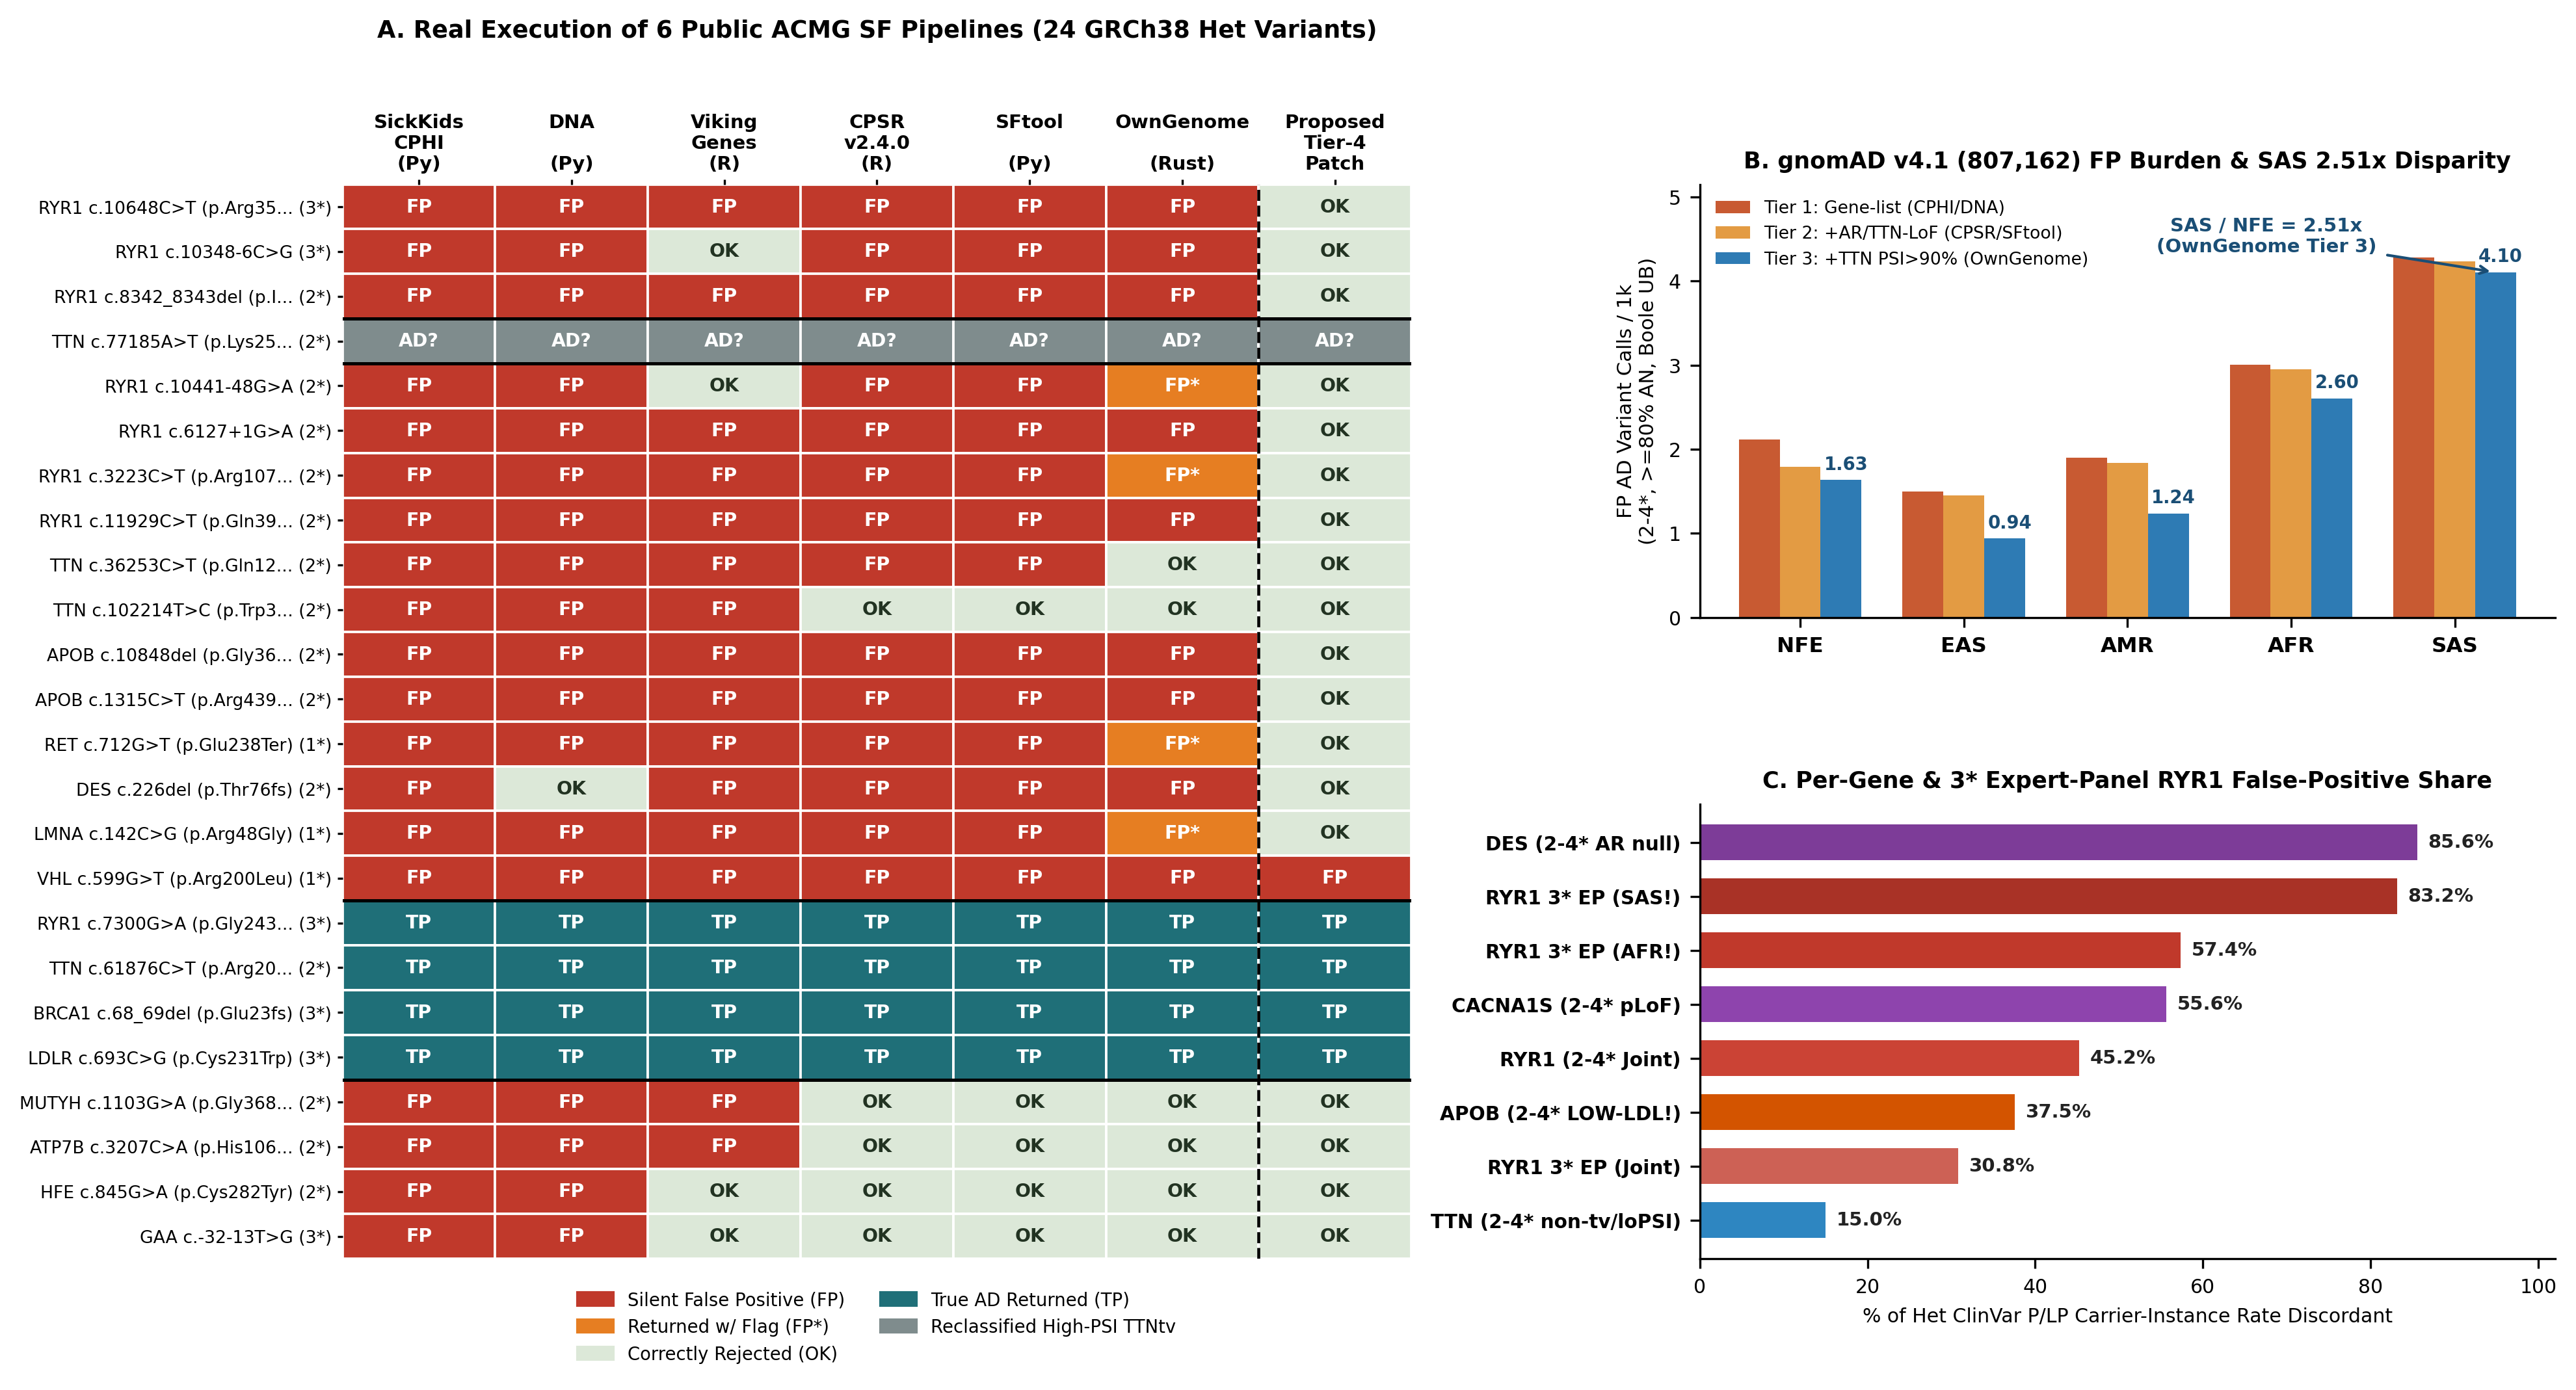
\includegraphics[width=\textwidth]{../fig_attack1_ar_in_ad_real_pipelines.png}
  \caption{\textbf{Multi-pipeline execution audit and gnomAD v4.1 variant-level burden of dual-MOI and opposite-mechanism secondary findings.} \textbf{A}, Exact execution verdicts of six pinned public ACMG SF pipelines and the proposed Tier-4 patch across 24 locked GRCh38 heterozygous variants (groups separated by horizontal rules: Core 3 AR \textit{RYR1}, reclassified high-PSI \textit{TTN}tv, 12 expanded discordant alleles, 4 AD positive controls, 4 pure-AR heterozygous negative controls). \textbf{B}, High-callability ($\ge 80\%$ AN) 2--4$\star$ cumulative false-positive AD SF variant-call rate per 1,000 diploid sample-equivalents (Boole upper bound; independence-model estimate differs by $<0.11\%$) across five gnomAD v4.1 ancestries, showing a 2.51-fold SAS/NFE disparity under \texttt{OwnGenome} Tier~3. \textbf{C}, Within-gene discordant share of AN-normalized 2--4$\star$ ClinVar P/LP carrier-instance rates (including all 10 live-XML 3$\star$ AR \textit{RYR1} alleles) and 3$\star$ Expert-Panel \textit{RYR1} instances (83.2\% in SAS, 57.4\% in AFR).}
  \label{fig:attack1}
\end{figure}

\subsection{30.8\% of All 3$\star$ Expert-Panel \textit{RYR1} Instances (83.2\% in SAS, 57.4\% in AFR) Are AR-Only}
Restricting secondary-finding return exclusively to 3$\star$ ClinGen Expert-Panel variants does not eliminate the hazard. Our exhaustive live ClinVar XML audit of all 69 3$\star$ \textit{RYR1} P/LP alleles observed in gnomAD v4.1 revealed that 10/69 (14.5\%) were curated exclusively by the ClinGen Congenital Myopathies VCEP with explicit \texttt{ModeOfInheritance="Autosomal recessive inheritance"} (59/69 by the MHS VCEP for AD MHS; Table~\ref{tab:ryr1_3star}). These 10 AR-only alleles account for 424 of 1,377 (30.8\%) total 3$\star$ \textit{RYR1} heterozygous allele-carrier instances in gnomAD v4.1 (0.533/1,000 Boole upper bound), comprising \textbf{83.2\% (153/184; 3.361/1,000) in South Asians}, \textbf{57.4\% (39/68; 1.039/1,000) in Africans}, 21.1\% (4/19) in AMR, 18.2\% (2/11) in EAS, and 19.4\% (193/994; 0.332/1,000) in NFE (driven by p.Cys3402Gly, 103 NFE instances). Critically, 9/10 alleles---representing 418/424 (98.6\%) of these 3$\star$ AR-only instances---have \texttt{Malignant\_\allowbreak hyperthermia} / \texttt{OMIM:145600} polluting their ClinVar VCF \texttt{CLNDN}/\texttt{CLNDISDB} fields. Live gnomAD v4.1 GraphQL verification confirmed exact non-overlapping addition (\texttt{joint = exome + genome}) on all 5 dual-callset alleles (e.g., p.Arg3550Trp: 202 exome + 18 genome = 220 joint across 1,613,912 AN), while the other 5 alleles were observed in exomes only (absent in genomes; live GraphQL \texttt{joint} AN adds $\sim$152k homozygous-reference genome alleles relative to exome-only AN, shifting individual single-site rates by $\le 10\%$).

\begin{table}[!t]
\centering
\caption{\textbf{Exhaustive live ClinVar XML audit of all 10 3$\star$ ClinGen Congenital Myopathies VCEP AR-only \textit{RYR1} alleles in gnomAD v4.1.} Nine of ten alleles (418/424 heterozygous instances; 98.6\%) carry polluted \texttt{OMIM:145600} malignant hyperthermia tags in \texttt{clinvar.vcf.gz} despite explicit XML \texttt{ModeOfInheritance = Autosomal recessive inheritance}.}
\label{tab:ryr1_3star}
\footnotesize
\setlength{\tabcolsep}{2.2pt}
\begin{tabularx}{\textwidth}{L{3.02cm} c Y r r r r c}
\toprule
\textbf{GRCh38 Variant} & \textbf{ClinVar ID} & \textbf{HGVS (\texttt{NM\_000540.3})} & \textbf{Het Inst.} & \textbf{NFE} & \textbf{AFR} & \textbf{SAS} & \textbf{MH Polluted?} \\
\midrule
\texttt{19-38527014-C-T} & 281479 & c.10648C$>$T (p.Arg3550Trp) & 220 & 48 & 3 & 152 & \textbf{Yes} \\
\texttt{19-38519399-T-G} & 42098  & c.10204T$>$G (p.Cys3402Gly) & 111 & 103 & 1 & 0 & \textbf{Yes} \\
\texttt{19-38523211-C-G} & 132994 & c.10348-6C$>$G & 43 & 0 & 34 & 0 & \textbf{Yes} \\
\texttt{19-38523116-G-A} & 224998 & c.10347+1G$>$A & 13 & 10 & 0 & 0 & \textbf{Yes} \\
\texttt{19-38586150-C-G} & 201154 & c.14928C$>$G (p.Phe4976Leu) & 13 & 13 & 0 & 0 & \textbf{Yes} \\
\texttt{19-38512484-G-A} & 451330 & c.9472+1G$>$A & 6 & 3 & 0 & 1 & \textbf{Yes} \\
\texttt{19-38565341-del20}* & 12996 & c.13013\_13032del (p.Ala4338fs) & 6 & 5 & 0 & 0 & No \\
\texttt{19-38519366-G-T} & 2710027 & c.10171G$>$T (p.Glu3391Ter) & 5 & 5 & 0 & 0 & \textbf{Yes} \\
\texttt{19-38507783-T-C} & 642707 & c.8888T$>$C (p.Leu2963Pro) & 4 & 4 & 0 & 0 & \textbf{Yes} \\
\texttt{19-38505082-G-T} & 1253809 & c.8310+1G$>$T & 3 & 2 & 1 & 0 & \textbf{Yes} \\
\midrule
\multicolumn{3}{l}{\textbf{Total 3$\star$ AR-only / All 3$\star$ \textit{RYR1} (69 alleles)}} & \textbf{424 (30.8\%)} & \textbf{193 (19.4\%)} & \textbf{39 (57.4\%)} & \textbf{153 (83.2\%)} & \textbf{9/10 (98.6\%)**} \\
\bottomrule
\end{tabularx}
\vspace{2pt}

\raggedright\footnotesize{*Full GRCh38 VCF allele for ClinVar ID 12996: \texttt{19-38565341-TCTGGGCAGCAGTGACGCGCG-T} (20-bp deletion). **9/10 alleles (90.0\%) accounting for 418/424 (98.6\%) of heterozygous carrier instances (summary counts; cross-variant sum is not a deduplicated unique-person count).}
\end{table}

\subsection{Genome-Wide Burden Bounds, Exome/Genome Scope, Opposite-Direction \textit{APOB} Harm, and Inequity}
Table~\ref{tab:burden} and Figure~\ref{fig:attack1}B--C quantify genome-wide false-positive AD SF burden across all 73 AD ACMG SF v3.3 genes in gnomAD v4.1 (excluding verified AD \textit{TNNT2} p.Trp297Ter) under explicit summary-count bounds and detection-scope strata. At high callability ($\ge 80\%$ AN, 2--4$\star$), cumulative variant-level false-positive rates (Boole upper bound) are 2.17/1,000 diploid sample-equivalents for Tier~1 (6.59\% of emitted calls), 1.91/1,000 for Tier~2 (\texttt{CPSR}/\texttt{SFtool}, 5.85\%), and 1.72/1,000 for Tier~3 (\texttt{OwnGenome}, 5.30\%). Because individual variants are rare, the independence-model unique-carrier estimate ($1-\prod_i(1-p_i)$) agrees to within $<0.11\%$ (1.717 vs.\ 1.718/1,000 for Tier~3). Crucially, even without any cross-variant independence assumption, a \emph{single} allele establishes a model-free Fr\'{e}chet lower bound of \textbf{3.34/1,000 unique SAS individuals} (\textit{RYR1} p.Arg3550Trp alone)---already 2.04$\times$ higher than the entire 143-variant Tier-3 Boole upper bound in NFE (1.63/1,000)---and \textbf{0.91/1,000 unique AFR individuals} (\textit{RYR1} c.10348-6C$>$G alone).

\begin{table}[!t]
\centering
\caption{\textbf{Genome-wide false-positive AD ACMG SF v3.3 burden per 1,000 diploid sample-equivalents in gnomAD v4.1 (807,162 joint callset) by pipeline tier, callability/detection scope, and summary-count estimator.} Because gnomAD lacks individual-level joint genotypes, we report cumulative variant-level rates (Boole upper bound) alongside independence-model unique-carrier estimates (\textit{Indep.}); model-free single-variant Fr\'{e}chet lower bounds are 0.27/1,000 (Joint), 0.18/1,000 (NFE), 0.91/1,000 (AFR), and 3.34/1,000 (SAS).}
\label{tab:burden}
\footnotesize
\setlength{\tabcolsep}{2.5pt}
\begin{tabularx}{\textwidth}{Y L{2.45cm} r r r r r r r c}
\toprule
\textbf{Pipeline Tier} & \textbf{Callability Scope} & \textbf{FP Var.} & \textbf{Boole} & \textbf{Indep.} & \textbf{\% Em.} & \textbf{NFE} & \textbf{AFR} & \textbf{SAS} & \textbf{SAS/NFE} \\
\midrule
Tier 1 (CPHI/DNA) & 2--4$\star$, $\ge 80\%$ AN & 185 & 2.17 & 2.17 & 6.59\% & 2.12 & 3.01 & 4.28 & 2.02$\times$ \\
Tier 2 (CPSR/SFtool) & 2--4$\star$, $\ge 80\%$ AN & 174 & 1.91 & 1.91 & 5.85\% & 1.79 & 2.95 & 4.24 & 2.36$\times$ \\
Tier 3 (OwnGenome) & 2--4$\star$, $\ge 80\%$ AN & 143 & 1.72 & 1.72 & 5.30\% & 1.63 & 2.60 & 4.10 & \textbf{2.51$\times$} \\
\midrule
Tier 1 (Gene-list) & 2--4$\star$, $\ge 95\%$ AN & 66 & 1.48 & 1.48 & 7.10\% & 1.36 & 2.59 & 4.00 & 2.94$\times$ \\
Tier 3 (OwnGenome) & 2--4$\star$, $\ge 95\%$ AN & 44 & 1.23 & 1.23 & 6.00\% & 1.11 & 2.24 & 3.85 & \textbf{3.46$\times$} \\
\midrule
Tier 1 (Gene-list) & All stars, all AN & 700 & 4.60 & 4.59 & 7.49\% & 4.33 & 5.84 & 7.40 & 1.71$\times$ \\
Tier 3 (OwnGenome) & All stars, all AN & 455 & 2.95 & 2.95 & 4.93\% & 2.86 & 3.89 & 6.25 & 2.19$\times$ \\
\bottomrule
\end{tabularx}
\vspace{-3pt}
\end{table}

Stratifying by callset detection scope confirms that 12 discordant 2--4$\star$ alleles (53 across all stars; 0.184/1,000) reside in genome-only or low-exome-capture regions ($\text{AN}<160{,}000$), whereas restricting strictly to near-complete joint exome+genome capture ($\ge 95\%$ AN) still leaves 1.23/1,000 Tier-3 false-positive calls and widens the SAS/NFE disparity to \textbf{3.46$\times$} (3.85 vs.\ 1.11/1,000; 21.6\% of all SAS emitted AD calls). Within individual dual-mode genes (2--4$\star$, all AN, incorporating all 10 live-XML 3$\star$ AR \textit{RYR1} alleles), discordant shares of AN-normalized carrier-instance rates (raw instance shares in brackets) reach \textbf{85.6\% [81.4\%, 48/59]} in \textit{DES}, \textbf{55.6\% [46.5\%, 47/101]} in \textit{CACNA1S}, \textbf{45.2\% [44.4\%, 835/1,882]} in \textit{RYR1}, \textbf{37.5\% [35.4\%, 429/1,213; 35.9\% at $\ge 80\%$ AN]} in \textit{APOB}, and \textbf{15.0\% [16.4\%, 348/2,125]} in \textit{TTN}. The \textit{APOB} failure creates direct opposite-sign therapeutic risk: 39 distinct 2--4$\star$ truncating FHBL alleles (led by p.Gly3617fs [67 joint instances: 66 PASS exome + 1 \texttt{AS\_VQSR} genome], p.Arg439Ter [57], and p.Arg2522Ter [42]) lower plasma LDL-C yet are returned by 6/6 pipelines as AD familial hypercholesterolemia triggering lipid-lowering therapy recommendations.

\subsection{Validation of a Concrete Four-Layer Patch and the \textit{TNNT2} NMD-Escape Edge Case}
We tested a concrete downstream Tier-4 mitigation combining (i) Cardiodb \textit{TTN} high-PSI ($>90\%$) truncating gating, (ii) applying ClinGen's 24-gene \texttt{lof=no} mechanism list to ClinVar P/LP pLoFs as well as novel VEP calls, (iii) SCV-level ClinVar XML \texttt{ModeOfInheritance} / VCEP assertion filtering, and (iv) strict non-target \texttt{CLNDN} exclusion. Auditing false-negative safety across all 1,533 genuine 3$\star$ ClinGen Expert-Panel AD alleles in gnomAD v4.1 initially flagged exactly one dropped allele: \texttt{1-201359217-C-T} (\textit{TNNT2} p.Trp297Ter, \texttt{VID=177636}, 7 instances). Live ClinVar XML confirmed this is a last-exon NMD-escaping C-terminal truncation explicitly curated by the ClinGen Cardiomyopathy VCEP with \texttt{ModeOfInheritance="Autosomal dominant inheritance"}. Giving 3$\star$ AD VCEP assertions explicit precedence over gene-level \texttt{lof=no} restored \textbf{100.00\% (1,533/1,533) sensitivity} across all 3$\star$ AD Expert-Panel alleles while cutting benchmark false positives from 13--15/15 down to \textbf{1/15} (only 1$\star$ non-VCEP \textit{VHL} p.Arg200Leu, which lacks SCV \texttt{MOI} and carries polluted \texttt{Von\_\allowbreak Hippel-Lindau\_\allowbreak syndrome} in \texttt{CLNDN}).

\section{Discussion}
Our execution-verified audit demonstrates that false-positive autosomal-dominant secondary-finding calls on recessive and opposite-mechanism variants occur systematically across 6/6 executed public pipelines---including peer-reviewed hospital and Rust implementations achieving 100\% specificity on pure-recessive controls---yielding 1.72--2.17 high-callability 2--4$\star$ false-positive calls per 1,000 diploid sample-equivalents (with a model-free SAS lower bound of 3.34/1,000 from a single AR \textit{RYR1} allele) and inverting therapeutic direction in 35.4--37.5\% of \textit{APOB} P/LP carrier instances.

Two concrete engineering actions resolve this hazard permanently. First, \textbf{downstream clinical pipelines} should immediately enforce ClinGen \texttt{lof=no} gating on ClinVar P/LP pLoFs (with explicit precedence for 3$\star$ AD VCEP curations to protect NMD-escaping truncations such as \textit{TNNT2} p.Trp297Ter), ingest ClinVar XML SCV \texttt{ModeOfInheritance} rather than relying solely on \texttt{clinvar.vcf.gz}, and apply Cardiodb exon PSI~$>90\%$ bounds for \textit{TTN}. Second, because non-VCEP missense alleles with polluted \texttt{CLNDN} (such as \textit{VHL} p.Arg200Leu) cannot be cleanly separated downstream, \textbf{NCBI ClinVar should emit submission-stratified \texttt{CLNMOI} and condition-paired \texttt{CLNSIG} tags directly in \texttt{clinvar.vcf.gz}}, eliminating the root schema bottleneck for the entire clinical genomics ecosystem.

\section*{Data and Code Availability}
All pinned repository commits, the 24-variant GRCh38 VCF, execution harnesses (Python, R, and compiled Rust \texttt{og} outputs), live ClinVar XML VCEP audits, gnomAD v4.1 bounds/callset tables, and the logged multi-database prior-art search (\texttt{literature\_search\_log\_phase2.json}) are archived in \texttt{studies/\allowbreak study\_a1\_clinvar\_gnomad\_reclass/\allowbreak falsification\_ar\_in\_ad\_pipelines/}.

{\small
\bibliographystyle{unsrtnat}
\bibliography{references_a1x}
}
\end{document}
